% !TeX root = ../main.tex
% !TeX encoding = UTF-8
% !TeX spellcheck = none
% 由05-main-results.tex加载，继续5.2的三级标题编号。
\subsubsection{不同常规模式偏离程度下的预测性能}\label{sec:scenario-performance}\label{sec:exp-scenarios}

总体指标与空间案例之外，分组评价进一步考察模型在常规模式偏离时的预测表现及残差作用。分析使用生成现有图件时锁定的模型，在成都和上海分别使用第118轮和第116轮的检查点。全部分组仅使用预测起点之前的12步观测，常规参考和分位数阈值由训练历史拟合后冻结；各方法共享测试窗口、组别及正目标值掩码。分组MAE在相应预测步的有效样本--网格位置上合并计算，批次补齐样本不参与统计。

对各网格和通道，以训练历史中同工作日/周末类型、同五分钟时间槽的流量中位数作为外部分析的常规参考。历史观测减去该参考后，除以按网格和通道从训练残差拟合的稳健尺度\(\max(1,1.4826\,\mathrm{MAD})\)，得到标准化残差；取历史12步残差绝对值的均值作为偏离分数。按训练分数的第50、80和95百分位数，将测试位置划分为Low、Moderate、High和Extreme四组。该外部分组参考用于解释预测结果，不改变模型输入、训练或检查点选择；分组细节见补充材料S1。

\begin{figure}[!htbp]
  \centering
  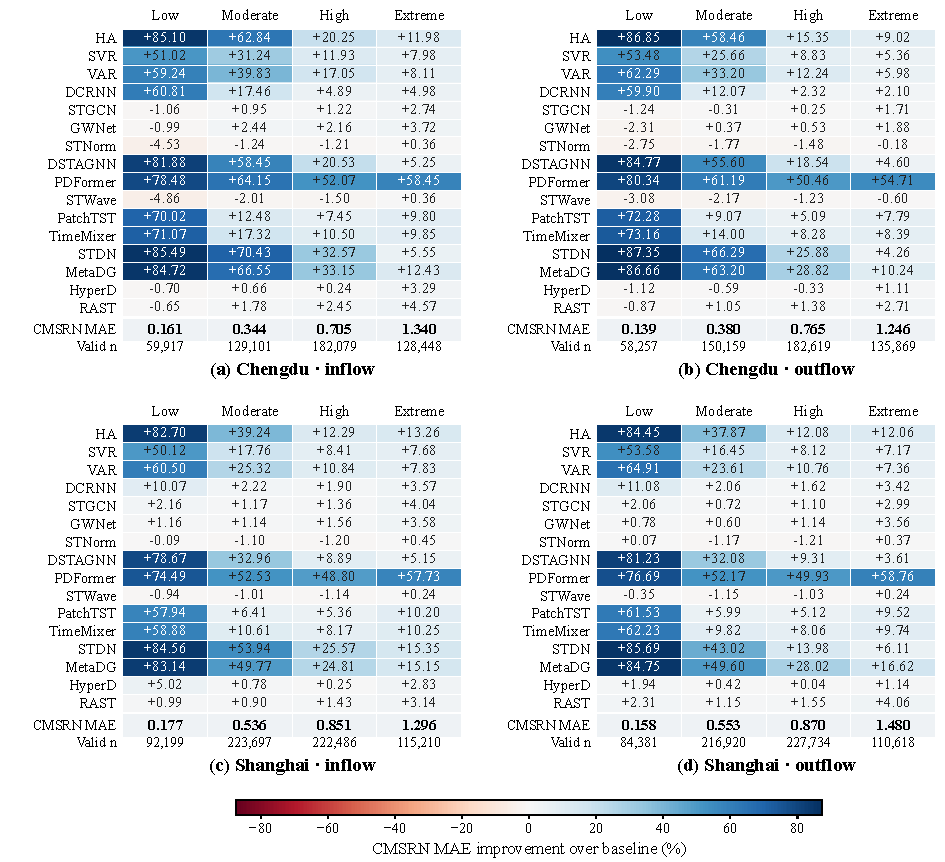
\includegraphics[width=\linewidth]{figures/scenarios/performance_h6_paper.pdf}
  \caption[常规模式偏离程度与H6预测性能]{\textbf{不同常规模式偏离程度下的H6预测性能。}四个面板对应成都和上海的流入、流出。单元格为\(100(\mathrm{MAE}_{m}-\mathrm{MAE}_{\mathrm{CMSRN}})/\mathrm{MAE}_{m}\)，正值（蓝色）表示CMSRN误差较低，负值（红色）表示相应基线误差较低。图中保留全部16种基线及统一色标；面板底部给出CMSRN的MAE和有效样本--网格数\(n\)。图内百分比保留两位小数。}
  \label{fig:scenario-performance}
\end{figure}

图~\ref{fig:scenario-performance}比较H6（提前30分钟）的分组表现。与总体结果表相比，情景分析另加入VAR、STNorm与STWave，构成16种基线的扩展比较。CMSRN在四项城市--通道任务中的MAE均随偏离等级升高而增大，但在Extreme组的相对排名更靠前：成都流入及上海两通道均排名第一，成都流出排名第三。前三项相对于最接近的基线STWave，MAE分别降低0.36\%、0.24\%和0.24\%；成都流出的MAE则比STWave高0.60\%。STNorm和STWave在多个较低偏离组中仍取得更低误差，表明CMSRN的相对竞争力具有情景和通道差异。

这一结果与本文关注局部流量偏离常规模式时的预测修正相呼应。与此同时，Extreme组的绝对误差仍较大，四项任务的MAE为Low组的7.32--9.38倍（补充图S1）。偏离等级还伴随流量规模变化，因此上述比较描述的是实际分组中的预测表现；其与残差通路的联系进一步由下述固定模型诊断考察。



\subsubsection{SERR在不同近期变化情景下的残差作用}\label{sec:scenario-serr}

在High与Extreme合并的高偏离子集中，以历史相邻标准化残差绝对差的均值描述近期变化强度，并按训练高偏离样本中该量的第75百分位数划分平缓变化（Slow）与快速变化（Rapid）两组。为考察已训练模型中各残差的实际作用，固定模型参数、门控和其余输出，分别从最终预测中扣除指定残差，计算
\begin{equation}
  \Delta\mathrm{MAE}_{e}
  =\mathrm{MAE}(\widehat Y-C_e)-\mathrm{MAE}(\widehat Y),
  \label{eq:scenario-residual-removal}
\end{equation}
其中\(C_e\)为实际加入预测的有符号修正量，包含门控、强度系数及逆标准化尺度。正值表示原残差降低了该组的平均MAE。该诊断与第\ref{sec:exp-ablation}节的独立重训练消融互为补充：前者度量锁定模型对既有修正的敏感性，后者比较重新训练后的修正通路配置。

图~\ref{fig:scenario-serr}中，两类专家在八个城市--通道--变化组上的16个移除差值均为正。自身残差在快速变化组的移除代价一致更大，为平缓组的1.61--2.82倍；例如，成都流入由0.0317增至0.0893，上海流入由0.0682增至0.1448。这说明，在当前高偏离样本中，节点自身演化修正在近期变化较快时对应更大的绝对MAE收益。时滞残差提供幅度较小的正向补充，其移除代价在成都的快速变化组增大，在上海则减小。两类角色呈现不同的情景响应，支持对自身动态与跨区域时滞信息分别组织修正证据。

\begin{figure}[!htbp]
  \centering
  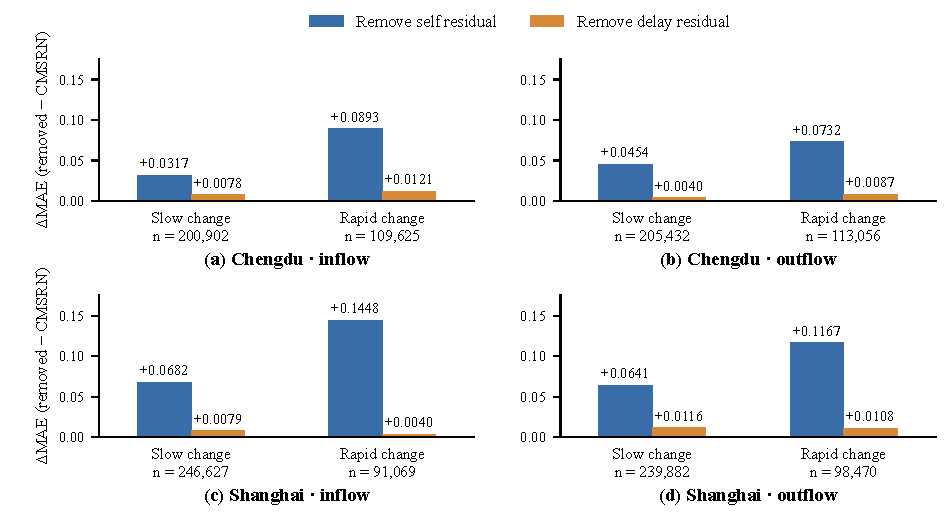
\includegraphics[width=0.92\linewidth]{figures/scenarios/serr_sensitivity_h6_paper.pdf}
  \caption[SERR在近期变化分组中的残差作用]{\textbf{高偏离情景下SERR的H6残差移除敏感性。}蓝柱和橙柱分别表示扣除自身残差与时滞残差后的\(\Delta\mathrm{MAE}\)，单位为原始5分钟流量计数；\(n\)为各组正目标样本--网格数。自身项扣除的是已加权的“自身预测减基础预测”修正。门控及其他残差保持不变，权重不重新归一化；两柱的MAE差值不具有可加性。}
  \label{fig:scenario-serr}
\end{figure}

\subsubsection{BCMS在不同背景差异与预测时距下的残差作用}\label{sec:scenario-bcms}

进一步在高偏离子集中，计算目标网格与各有效固定候选网格的历史平均标准化残差之差的绝对值，再对候选取均值，作为候选背景差异。使用训练高偏离样本的三分位阈值划分Low、Medium和High三组。该量由历史流量构造，是分析用的背景代理，并非BCMS内部学习到的低频表征。沿用式~\eqref{eq:scenario-residual-removal}，在H1--H12分别扣除完整BCMS修正，检查其作用随背景条件与预测时距的变化。

图~\ref{fig:scenario-bcms}显示，对每个城市、通道和预测步，低背景差异组的平均修正收益均高于中等组，中等组又高于高差异组。例如，上海流入在H6的三个\(\Delta\mathrm{MAE}\)依次为0.012448、0.008885和0.006301。144个背景组--预测步单元中有143个为正，唯一负值为成都流出高背景差异组H5的约\(-4.8\times10^{-6}\)。各组收益随预测步波动，未呈现随时距单调增加的规律。这些结果表明，BCMS的平均修正作用与候选背景条件有关，并在背景代理较接近的样本中更大。

将分析扩展至完整测试集后，各对应背景组--预测步的平均收益均高于高偏离子集，且仍保持低差异组高于中、高差异组的顺序（补充图S2）。例如，上海流入低背景差异组H6的\(\Delta\mathrm{MAE}\)由0.012448增至0.023927，表明BCMS的有效补充也覆盖其他交通状态。结合SERR的分组响应，自身演化修正在快速变化样本中具有更大的绝对MAE收益，而跨区域消息补充在背景代理较接近的样本中更有效。

\begin{figure}[!htbp]
  \centering
  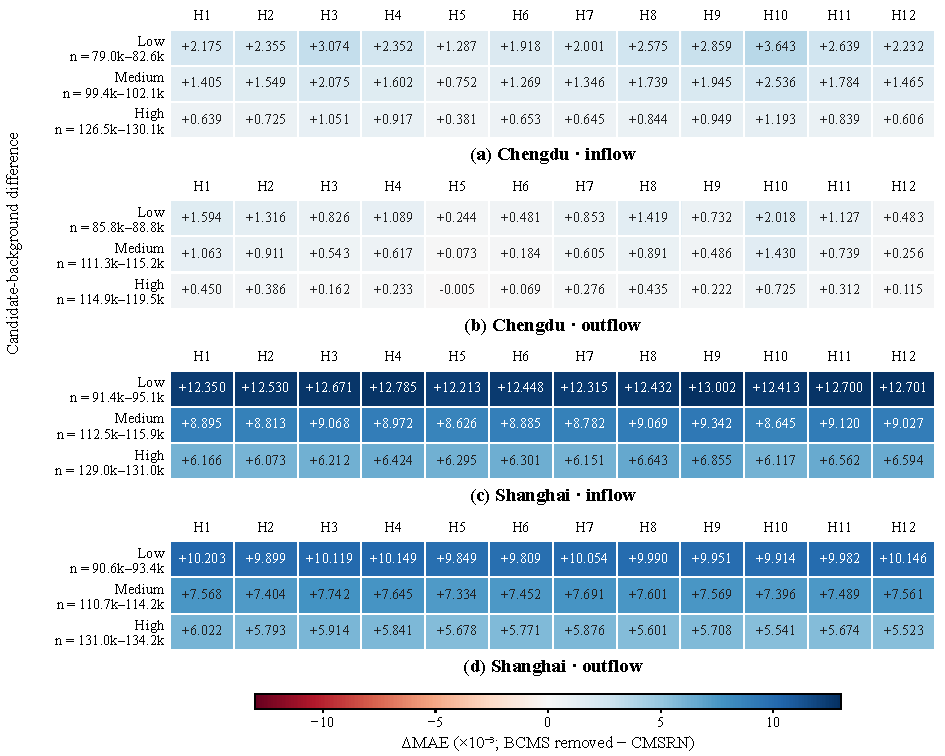
\includegraphics[width=0.92\linewidth]{figures/scenarios/bcms_sensitivity_horizons_paper.pdf}
  \caption[BCMS在背景差异与预测步分组中的残差作用]{\textbf{高偏离情景下BCMS的背景差异--预测步敏感性。}每格表示固定其余输出后扣除BCMS残差引起的MAE变化，数值按\(10^{-3}\)为单位显示，即图示值为\(1000\times\Delta\mathrm{MAE}\)。正值表示原修正降低组平均误差；H1--H12对应5--60分钟。背景组跨预测步保持固定，\(n\)的范围来自各步正目标位置数量的变化。该图为固定模型的输出移除诊断。}
  \label{fig:scenario-bcms}
\end{figure}
